\setstretch{1.0}
\chapter{An Atlas Based Approach for Whole Brain Functional Network Analysis}\label{chap_atlas}

In the previous experimental chapters we have introduced methods for investigating functional connectivity in large cortical volume. However as powerful as these methods are, they are fundamentally limited to investigating relations between two ROIs, and so overlook much the brain volume. In this chapter we propose an alternative method, which investigates functional connections simultaneously across the entire brain volume, albeit at the expense of spatial resolution by parcellating the brain into multiple distributed ROIs. Also, previous network analyses both undertaken in this thesis and other studies look for brain regions that share a common temporal profile of \textit{activity}. Here distinctly, we measure the temporal evolution of connectivity between pairs of parcellated brain regions and then use temporal ICA to uniquely identify networks of \textit{connections} whose temporal dynamics covary. We validate our method using MEG data recorded during a finger movement task, identifying a transient network of connections linking primary motor and motor planning regions, which modulates during the task. Next, we use our method to image the networks which support cognition during a Sternberg working memory task. We generate a novel neuroscientific picture of cognitive processing, showing clearly the formation and dissolution of multiple networks which relate to semantic processing, pattern recognition and language as well as vision and movement. In summary, our method offers an original means to track the dynamics of brain networks on a timescale commensurate to the task they are undertaking.

\doublespacing

\section*{Introduction}
In Chapters \ref{chapter_cca} and \ref{chap_kmeans}, we introduced novel multivariate methods to investigate functional connectivity over 5 dimensions. We then applied them to group studies (within the senorimotor network) to reveal new modes of connectivity. The results are important as they confirm that the resting state networks are temporal aggregates of much smaller, transient subnetworks which can be characterised with functional tasks. The methods used in those chapters should be transferable to other resting state networks and reveal their functional constituents or even cross network relations (such as those assessed by \citealp{Fox2005} for example) at high spatial resolutions. However, as powerful as this method is, it does have its limitations. First, it is limited to comparing two cortical volumes to each other, which poses questions about how you assess connections in networks with > 2 major ROIs. For example, the DMN can be crudely split into 4 functional hubs, the posterior cingulate cortex (PCC),  the medial prefrontal cortex (mPFC) and the angular gyri (LAG, RAG), so placing a seed in the PCC and the test as the other hubs will reveal connections which rely on the PCC but neglect for example a connection which exists exclusively between the the LAG and mPFC. For this multiple instances of CCA would need to be applied across all node combinations. this is not necessarily a problem to compute, but it runs the risk of producing 'too much data' to be able to infer all connections and their behaviours. Secondly CCA does not cover the entire the brain volume; whilst it could be suggested that you could compare the left and right hemispheres to each other, you can only assess the bilateral connections and neglect intrahemispheric relations (for example frontoparietal connections).  

It could be suggested that it is possible to assess every voxel timecourse to every other in a mass univariate test, giving us connectivity information for between every voxel pair. However this has many drawbacks. For example if our brain has 4000 voxels, a $4000 \times 4000$ array of data uses $\sim$120 MB which limits the number of windows of connectivity which can be stored in RAM in a high-end workstation to around 300. Secondly, trying to correct the leakage between 4000 voxels is raises the question of how to best approach this (though a method has been proposed by \citep{Maldjian2014}). Finally the smoothness of MEG data would lead to a large amount of redundancy in the results being presented. A solution to this problem is to break down the entire brain into regions larger than voxels, a process known as parcellation. These parcels typically represent a local region which shares a similar anatomical or functional profile, so are often derived from either decomposition of functional data or from an anatomical atlas. Post parcellation it is possble to extract timecourses representative to those parcels and assess connectivity between those instead. This allows for a general representation of connectivity across the brain, but at the cost of spatial specificity. This method has proven popular in recent studies \citep{Allen2014,Bola2015,Colclough2015,Finn2015,Hassan2015,Hillebrand2012,Smith2015,Tewarie2014a}. In this chapter, we propose a novel pipeline to assess dynamic functional connectivity between multiple ROIs distributed across the whole brain. We combine the approach of cortical parcellation with the recently developed symmetric orthgonlisation \citep{Colclough2015} method of leakage correction and sliding windows to capture the time evolving connections across the brain volume. 

One of the most useful tools to elucidate networks from inferred timecourses has been independent component analysis (ICA). For example, in MEG, the amplitude envelopes of band limited signals (representing brain ‘activity’) are acquired from multiple voxels and decomposed into a smaller number of temporally independent components, with a single component representing temporal signatures at multiple voxels. Assessment of the voxels contributing to each component thus yields networks of regions which share a temporal profile (\citealp{Brookes2011,Luckhoo2012,Hall2013}; Chapter \ref{sec_bf_v_mn}). Here, distinct from this, having characterised the timecourse of electrophysiological connectivity between region pairs, we apply ICA to timecourses of \textit{connectivity}. In other words, ICA is applied such that a single component represents a temporal signature shared by multiple connections. Assessment of the connections contributing to each component then yields a spatial pattern representing a network of connections. In this way, we uniquely track the dynamic behaviour of networks, on a timescale commensurate to the task they are undertaking without having to assess networks individually like in Chapter \ref{chap_kmeans}. We will use this method to generate a novel neuroscientific picture of task evoked cognitive processing. In Section \ref{sec_atlas_methods} we introduce the processing pipeline which allows us to investigate dynamic whole brain connectivity. We then apply this to two individual studies in Section \ref{sec_atlas_results}.

\section{Methods}\label{sec_atlas_methods}
\subsection{Data Acquisition}
Two separate MEG datasets were acquired. Ethical approval for both studies were granted by the University of Nottingham Medical School Research Ethics Committee.
\begin{itemize}
\item \textbf{Dataset 1} -- \textit{Self Paced Motor task:} 10 volunteers (8 male, aged 25\pm 4 years (mean\pm SD)) were asked to execute a button press with the index finger of their non-dominant hand. Subjects were instructed to press the button infrequently (approximately once every 30 seconds) but not to count the time between presses. These data have also been used in Chapter \ref{chap_kmeans}. 
\item \textbf{Dataset 2} -- \textit{Sternberg Task:} 19 healthy participants (10 male, aged 25\pm 3 years) performed a Sternberg working memory task. Two example visual stimuli (abstract geometric shapes) were presented on a screen; each stimulus was shown for 0.6s with 1s between onsets. Following this, a period of 7 seconds was left, known as the maintenance phase, before a third (probe) stimulus was presented. If the probe stimulus matched either of the two example stimuli, the subject was told to execute a button press with their right index finger. Subjects received immediate feedback as to whether their response was correct. Trials were separated by 30 seconds of rest, where subjects fixated on a cross. 30 trials were presented per subject. \textit{Note that this Sternberg study is a different from that in Chapter \ref{chap_kmeans}}.
\end{itemize}

MEG data were recorded using a CTF MEG system in Nottingham according the protocols described in Chapter \ref{sec_data_acq}.

\subsection{Pre-processing and Source Reconstruction}
A schematic of the subsequent data processing pipeline is given in Figure \ref{fig_6_1}. 

Following pre-processing, data were analysed using beamforming. The cortex was parcellated using the Automated Anatomical Labelling (AAL) atlas \citep{Tzourio-Mazoyer2002} which had been modified by removing subcortical ROIs to leave 78 regions \citep{Gong2009}, and was transformed to each individual’s brain geometry using FMRIB Linear Image Registration Tool (FLIRT) in FSL \citep{Jenkinson2012}. In order to obtain a representative time-series for every region, the centre of mass of each region was defined and used as a single representative location for that region (Figure \ref{fig_6_1} – step 1). MEG data were frequency filtered 1-150 Hz and source localised using an adaptive beamformer \citep{VanVeen1997, Robinson1999} in order to derive 78 source timecourses per subject, one for each AAL region (Figure \ref{fig_6_1} – step 2). For beamforming, data covariance was defined in a frequency window spanning 1-150 Hz and a time window covering the entire experiment \citep{Brookes2008}. The covariance matrix was regularised using the Tikhonov method with the regularisation parameter set to 0.01 times the maximum eigenvalue of the unregularised matrix. Forward fields were based upon dipole approximations \citep{Sarvas1987} and a multiple local spheres head model \citep{Huang1999}. Dipole orientation was determined using a non-linear search for the optimal signal to noise ratio (SNR). This process creates a source space data matrix, \textbf{Q} of dimension $n_n \times n_s$, where $n_n$ is the number of AAL regions (=78) and $n_s$ is the number of time samples.

\begin{figure}[h!]
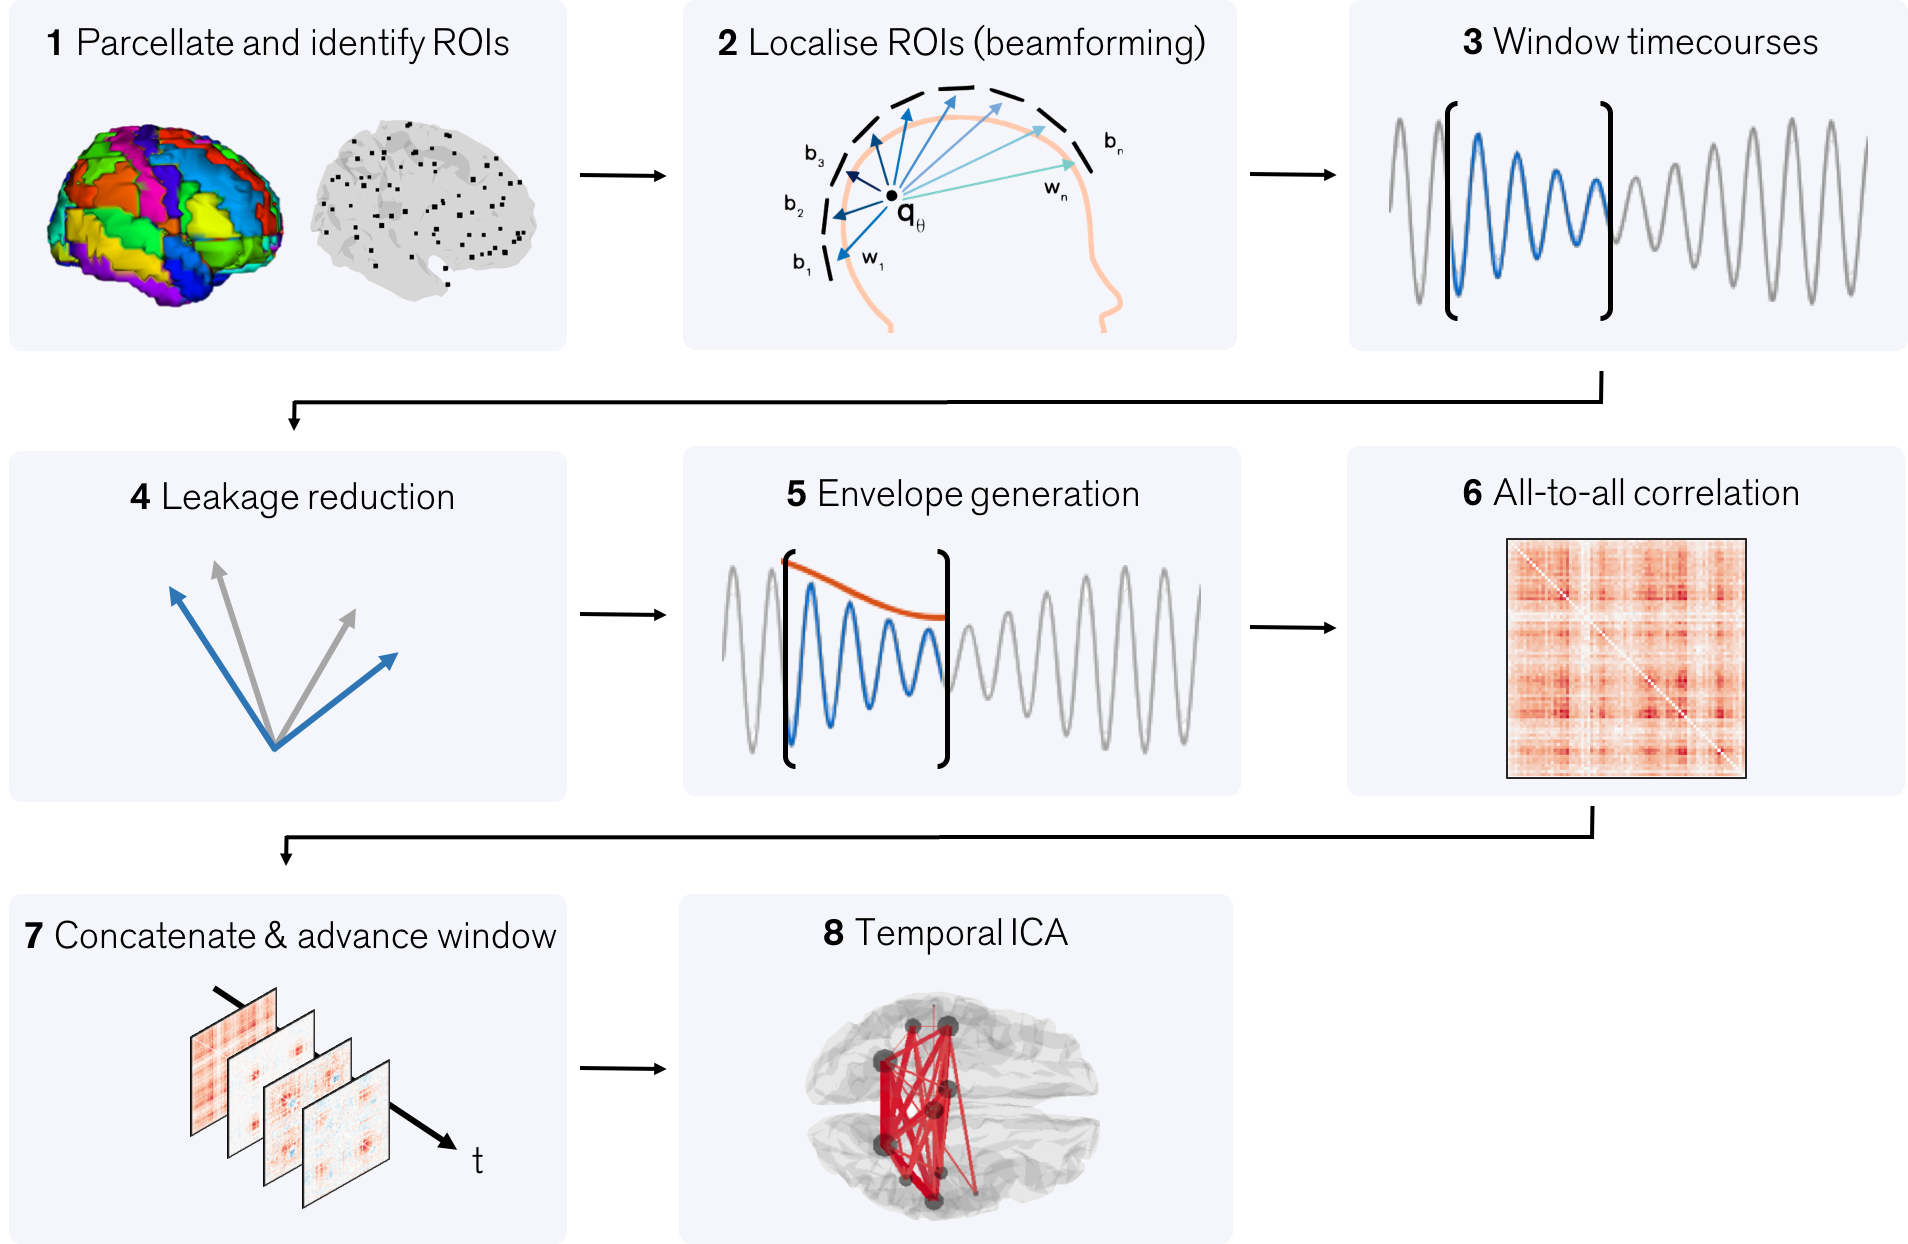
\includegraphics[width=\linewidth]{images/chapter6/figure_1.png}\caption{A schematic diagram describing the fundamental processing pipeline.}\label{fig_6_1}
\end{figure}

\subsection{Dynamic Functional Connectivity Analysis}
We aimed to undertake a dynamic, all-to-all, functional connectivity analysis. This means that connectivity between all possible pairs of AAL regions is measured, as a function of time, using a sliding window approach. Previous work \citep{Hipp2012, Baker2014} has shown that functional connectivity is dependent on frequency band studied; so to capture as many of the connections possible, we did not limit ourselves to a single established frequency band but rather looked to encompass as many frequencies as possible. We employed a 4-30 Hz frequency window, so as to cover the wide range of frequencies seen to be modulated in working memory paradigms \citep{Brookes2012a}. After frequency filtering, \textbf{Q} was segmented into overlapping time windows (Figure \ref{fig_6_1} – step 3): we denote the data in a single window, $\mathbf{Q}_i$, which has dimensions $n_n\times f\delta$. Here, $i$ denotes window number, $\delta$ is the window width in seconds, and $f$ is sampling frequency. In everything that follows $\delta$ = 6 s; the window was shifted in time by 0.5 s for each window number ($i$). In the self-paced motor task, time windows were centred between $t$ = -12 s and $t$ = 12 s (where $t$ represents window centre relative to the button press). There were 49 time windows per trial. In the Sternberg task, time windows were centred between $t$ = -13 s and $t$ = 25 s ($t$ represents window centre relative to trial onset). There were 75 time windows per trial. Within each window, we measured connectivity between all pairs of AAL regions.

To reduce the effect of the ill-posed nature of the source reconstruction artefactually inflating connectivity levels between ROIs we applied leakage reduction to the data. In the context of a multiple ROI dataset, a pairwise orthogonalisation technique could be sequentially applied between ROI pairs, but this raises the question as to which order the sequence should be applied. An elegant means to achieve orthogonalisation simultaneously over a set of multiple brain regions was recently proposed by  \cite{Colclough2015}. Here, signals from all $n_n$ regions are symmetrically orthogonalised within a single computation. The mathematical details of this procedure can found elsewhere (c.f \citealp{Colclough2015} for a full proof or Section \ref{sec_symm_orth} for the implementation used in this thesis). We applied symmetric orthogonalisation to each windowed data matrix $\mathbf{Q}_i$; the result is a set of matrices, $\mathbf{O}_i$, whose rows contain the orthogonalised (windowed) time series for all 78 AAL regions (Figure \ref{fig_6_1} – step 4). Note that the leakage reduction step was applied on each window separately (separate orthogonalisation for each $i$), rather than on the whole time series. This is because Chapter \ref{chap_kmeans} has shown that leakage depends on signal to noise ratio, which changes in different time windows.

Following leakage correction, the amplitude envelopes of the windowed timecourses were found using Hilbert transformation. This resulted in a set of matrices $\mathbf{E}_i$ whose rows contained the amplitude envelopes of orthogonalised neural oscillations (i.e. the envelope of the rows of $\mathbf{O}_i$; Figure \ref{fig_6_1} – step 5).  Following this, Pearson correlation between amplitude envelopes was measured to form connectivity matrices, $\mathbf{R}_i$, such that

\begin{equation}
\mathbf{R}_i = 
	 \begin{bmatrix}
		r(\mathbf{e}_{i1},\mathbf{e}_{i1}) & \hdots & r(\mathbf{e}_{i1},\mathbf{e}_{in_n}) \\
		\vdots & \ddots & \vdots \\
		r(\mathbf{e}_{in_n},\mathbf{e}_{i1}) & \hdots & r(\mathbf{e}_{in_n},\mathbf{e}_{in_n})
	\end{bmatrix},
\end{equation} where $\mathbf{e}_{ik}$ represents the vector of timecourse measurements in the k\textsuperscript{th} row of  and $r(x,y)$ represents the Pearson correlation coefficient between $x$ and $y$. In other words, $\mathbf{R}_i$ represents an $n_n \times n_n$ adjacency matrix representing connectivity between all AAL region pairs, in time window $i$ (Figure \ref{fig_6_1} – step 6). This process was repeated for all $i$, resulting in a set of $N$ matrices (one for each time window used) and then concatenated to form an adjacency tensor, \textbf{R}.

\subsection{Temporal ICA}
The adjacency tensor, \textbf{R}, measures the temporal evolution of functional connectivity between all pairs of AAL brain regions. We now seek to apply ICA to derive independent temporal signatures of connectivity. We begin by reshaping each $n_n \times n_n$ matrix into a $1\times n_n^2$ row vector. Then, noting that the inherent diagonal symmetry in the adjacency matrix leads to redundancy, we remove that redundancy to generate the $1\times n_c$ vector $\mathbf{\rho}_i$, where $n_c = \frac{n_n^2-n_n}{2}$ is the total number of unique connections modelled in $\mathbf{R}_i$. These multiple row vectors are then concatenated in time (Figure \ref{fig_6_1} – step 7) to generate a new matrix $\mathbf{\Rho}$ such that $\mathbf{\Rho} = [ \mathbf{\rho}_1 , \mathbf{\rho}_2 , \hdots , \mathbf{\rho}_N]^T$. This means that each column of $\mathbf{\Rho}$ represents the timecourse of an individual connection between 2 AAL regions. We then use ICA to decompose this matrix into a smaller number of temporal components. If we generate $n_{IC}$ independent components then

\begin{equation}
\hat{\mathbf{\Rho}}^T = \mathbf{AX}, \label{eqn_6_2}
\end{equation} where the rows of the $n_{IC} \times N$ matrix \textbf{X} represent temporally independent signatures of functional connectivity, collapsed across all connections. The mixing matrix, \textbf{A}, has dimension $n_c \times n_{IC}$ and each column represents the contribution of each individual connection to the independent component. The ‘hat’ notation in Equation \ref{eqn_6_2} denotes that $\hat{\mathbf{\Rho}}$ is an estimate of $\mathbf{\Rho}$ based upon the derived independent components. Here, $\mathbf{\Rho}$ was formed by concatenating all time windows, including all trials and subjects. The ICA decomposition was performed using the fastICA method \citep{Hyvarinen1999} using a deflation approach with $n_{IC}=10$. The spatial signature of each derived independent component was reconstructed based upon the columns of \textbf{A} (Figure \ref{fig_6_1} – step 8). It is important to note that ICA necessarily assumes non-Gaussianity\footnote{This may intially seem at odds with the requirement that data needs to be Gaussian for leakage correction to correctly operate, but in practice, the transformations from MEG data to MEG amplitude envelopes to correlation timecourses makes the timeseries no longer Gaussian}, which after assessing the kurtosis of the timecourses contained in the connectivity tensor (average$\pm$SD the self paced and Sternberg experiments are 3.04$\pm$0.12 and 2.99$\pm$0.12respectively), is reflected in the connectivity data itself.

\subsection{Testing for task-modulated networks}
The above analyses yields a set of $n_{IC}=10$ networks, showing functional connections that share similar (independent) temporal profiles. The challenge now becomes to determine which of these represent genuine brain networks. The question of which independent components reflect genuine brain processes and which reflect only noise is a problem in all ICA based methods. Here for simplicity, we sought to determine which networks were modulated significantly by the tasks. Our procedure was based, in part, on an algorithm previously used in fMRI \citep{Clare1999}. Specifically, we reasoned that if no task induced response was expected, then the trial onset times would be meaningless. Under this null hypothesis (assuming $N_t$ trials) the temporal modulation of the trial average timecourse representing a specific network would be no greater than a ‘sham trial average’ in which an equivalent number ($N_t$) of temporal epochs were considered, but with the ‘trial onsets’ chosen at random.  

In order to generate a trial averaged timecourse, the concatenated connectivity matrix, $\mathbf{\Rho}$, was reshaped and averaged across trials to generate a new matrix, $\bar{\mathbf{\Rho}}$, where the ‘bar’ notation represents a trial average. The size of this matrix was $\frac{N}{N_t}\times N_c$  (where $\frac{N}{N_t}$ represents the number of time windows per trial; 49 for the self-paced task and 75 for the Sternberg task). Note that $\bar{\mathbf{\Rho}}$ represents the time evolution of all connections in the brain throughout the average trial. Following this, linear regression was used to derive the contribution of each network (represented in the columns of \textbf{A}) to each time point in the trial average data, $\bar{\mathbf{\Rho}}$. Mathematically, if

\begin{equation}
	\bar{\mathbf{\Rho}} = 
	\begin{bmatrix}
		\bar{\mathbf{\rho}}_1 \\ \bar{\mathbf{\rho}}_2 \\ \vdots \\ \bar{\mathbf{\rho}}_{\frac{N}{N_t}}
	\end{bmatrix},
\end{equation} where $\bar{\mathbf{\rho}}_j$ represents the trial averaged connections at time point $j$, we then let

\begin{equation}
	\bar{\mathbf{\rho}}_j^T = \mathbf{A}\mathbf{\beta}_j+\mathbf{\epsilon}_j.
\end{equation} Here, the parameters in the vector, $\mathbf{\beta}_j$ represent the contribution of each ICA derived network to time point $j$ in the trial averaged data.  represents error (i.e. variance in $\bar{\mathbf{\rho}}_j^T$ not explained in \textbf{A}). We use $j$ to represent time point as distinct from $i$ above because $i$ represents time over the entire experiment, whilst $j$ represents time within the trial average. $\mathbf{\beta}_j$ was estimated as $\hat{\mathbf{\beta}}_j=\mathbf{A}^+\bar{\mathbf{\rho}}_j^T$, where $\mathbf{A}^+$ represents the pseudo-inverse of \textbf{A}.

In order to test for statistical significance, the above procedure was repeated. However rather than the trial averaged data ($\bar{\mathbf{\Rho}}$) defined based on genuine trial onsets (defined as 12s prior to the button press in the self-paced study and 13s prior to the onset of the Sternberg task in the Sternberg data), a ‘sham’ averaged dataset, $\tilde{\mathbf{\Rho}}$, was defined based on randomly selected ‘sham trial onsets’. Note the ‘tilde’ notation represents a sham trial averaged result. The linear regression procedure was used as described above, but noting that the derived parameters, $\tilde{\mathbf{\beta}}_j$, were now representative of an empirical null distribution. 4000 realisations of  $\tilde{\mathbf{\beta}}_j$ were generated, based on 4000 sets of sham trial onsets. The genuine timecourses, $\mathbf{\beta}_j$, were then compared to the empirical null distribution, $\tilde{\mathbf{\beta}}_j$. A significant result was determined if, within some time window of interest and for any given network, $\mathbf{\beta}_j$ was outside the 95\textsuperscript{th} percentile range of the null distribution (i.e. $p<0.05$). Time windows of interest were taken as the point in the trial at which the button was pressed (for the self-paced motor data) and the period encompassing the Sternberg task (in the case of the Sternberg data). The threshold for significance was Bonferroni corrected for multiple comparisons across 10 independent components (for both tasks) and across independent time windows (2) in the Sternberg data. A 2-tailed distribution was allowed, meaning that $\mathbf{\beta}_j$ could be both greater than, or less than the null distribution.

It is noteworthy that the above testing only looks for significance across the group of subjects. This test is robust, but takes no account of cross subject variance. This potentially means that the result could be driven by one, or a small number, of subjects. For this reason, we also performed a ‘split half’ analysis. This was identical to the statistical analysis above, but run on only half of the subjects (5, for the self-paced study and 10 for the Sternberg study). This was done a number of times, with a different set of subjects selected each time. We then tested, empirically, the cross subject variance by examining the variability when separate sets of subjects were used in the analysis.

\section{Results}\label{sec_atlas_results}
Figure \ref{fig_6_2} shows the results of our method applied to the self-paced data. Although 10 independent components were derived, here we present only the single network that demonstrated significant task modulation (in both the statistical test and the split half analysis). The other 9 networks are shown in Appendix \ref{sec_atlas_appendix_A}. Figure \ref{fig_6_2}A shows a matrix representation of the network. The ordering of the 78 AAL regions is overlaid for reference. Figure \ref{fig_6_2}B shows the same network represented in 3D and thresholded (70\% of the maximum connection strength) for clarity. Both the matrix and 3D visualisation show clearly that the network is centred on the right postcentral gyrus (right primary motor cortex) and highlights strong connections with the right premotor area, the supplementary motor regions and left primary motor cortex. Figure \ref{fig_6_2}C shows the time evolution of this network, averaged across trials (i.e. the black trace represents $\mathbf{β}_j$ averaged across all subjects). The grey area represents the null distribution ($\tilde{\mathbf{β}}_j$) and the vertical line shows the time of the button press. Note the significant modulation of connectivity during the task. Figure \ref{fig_6_2}D shows the result of our ‘split-half’ analysis. Here, the black line represents the average response across groups of 5 subjects (as distinct from the average over 10 subjects shown in Figure \ref{fig_6_2}D). The blue shaded region shows the 90\textsuperscript{th} percentile (i.e. 90\% of all combinations of 5 subjects fall within this area) and therefore represents variability across subjects. The grey region shows the null distribution (for 5 subjects). Note that times at which the blue shaded region and grey region no longer overlap represent points at which 95\% of combinations of 5 subjects show a significant task induced modulation. Overall, it is clear that a plausible network representing primary and planning motor regions are modulated significantly by the button press.

\begin{figure}[h!]
	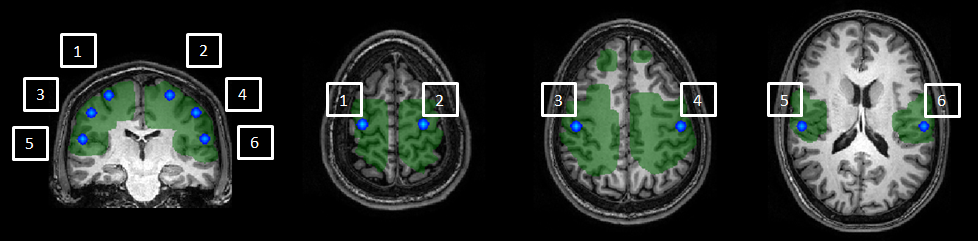
\includegraphics[width=\linewidth]{images/chapter6/figure_2.png}\caption{Results of the self-paced experiment. A) Matrix representation (unthresholded) of the network; the ordering of the 78 AAL regions is overlaid. Note that the values in the matrix are the ICA derived mixing coefficients. B) 3D representation of the same network, thresholded for visualisation. Lines show connections, with thicker lines indicating stronger connections. Circles represent the summed magnitude of connectivity between that region and the rest of the brain. C) Time evolution of the network during the self-paced task, averaged across trials in all subjects (black line). The grey shaded region represents the null distribution; significance (\textit{p}\textsubscript{corrected}<0.05) is attributed if the black line appears outside the null distribution during the task (at $t = 0$). D) Split-half analysis showing the mean response across groups of 5 subjects (black line). The grey shaded area represents the null distribution (for 5 subjects) and the blue shaded area shows variability between subjects. Note that the network clearly represents the primary motor, pre-motor and supplementary motor regions and demonstrates significant modulation with the task.}\label{fig_6_2}
\end{figure}

Figure \ref{fig_6_3a}-B shows the results of the same method applied to our Sternberg dataset. Clearly, the increased cognitive load evoked by the Sternberg tasks elicits changes in a greater number of brain networks, and this is shown by 9 of the 10 networks derived demonstrating significant task induced modulation. Figure \ref{fig_6_3a}-B is laid out such that the columns represent: (A) a 3D network visualisation, (B) the average timecourse (19 subjects) and (C) the split-half analysis. The separate rows (I through IX) show the 9 networks which modulate significantly.

Unsurprisingly given the visual nature of the task, the four networks showing early task modulation all involve the visual areas. These are shown in rows I to IV of Figure \ref{fig_6_3a}. Specifically, row I depicts a primary visual network whose connectivity increases during presentation of the two example stimuli (and also during the probe). Rows II and III show right and left lateralised connections between the primary visual areas and tempero-parietal regions, with both networks exhibiting an early increase in connectivity peaking immediately before presentation of the example stimuli. Row IV shows a visual to right motor cortex connection, which demonstrates a significant drop in connectivity during presentation of the example stimuli. Transient networks forming in later task phases are shown in rows V to IX in Figure \ref{fig_6_3b}. Row V shows a breakdown in connectivity during the task maintenance phase within a bilateral parietal, temporal and frontal network. Interestingly, this network captures some areas associated with the default mode network whose activity is known to decrease with a cognitive task. However, the network also captures areas associated with semantic processing and is thus termed the semantic network. Row VI highlights a left lateralised network that incorporates regions of temporal, parietal and frontal cortex. The regions implicated are strongly associated with the production of language as well as shape and pattern recognition; this is consistent with peaks in connection strength occurring during presentation of the stimuli. Row VII shows a refined visual to temporal and parietal network, similar to that in III but this time peaking around the time of the probe stimulus. Row VIII again shows a visual to motor connection (similar to IV), and finally row IX shows the sensorimotor network which becomes most strongly connected around the time of the button press response (in agreement with our result in Figure \ref{fig_6_2}). It is noteworthy that the brain regions implicated in these networks incorporate the primary sensory cortices, association areas, and cognitive networks that would be associated with somantic processing, pattern recognition and verbalisation, and so these networks are highly plausible given the task. This is addressed further in our discussion.

\clearpage

	\begin{figure*}[h!]
		\begin{center}
			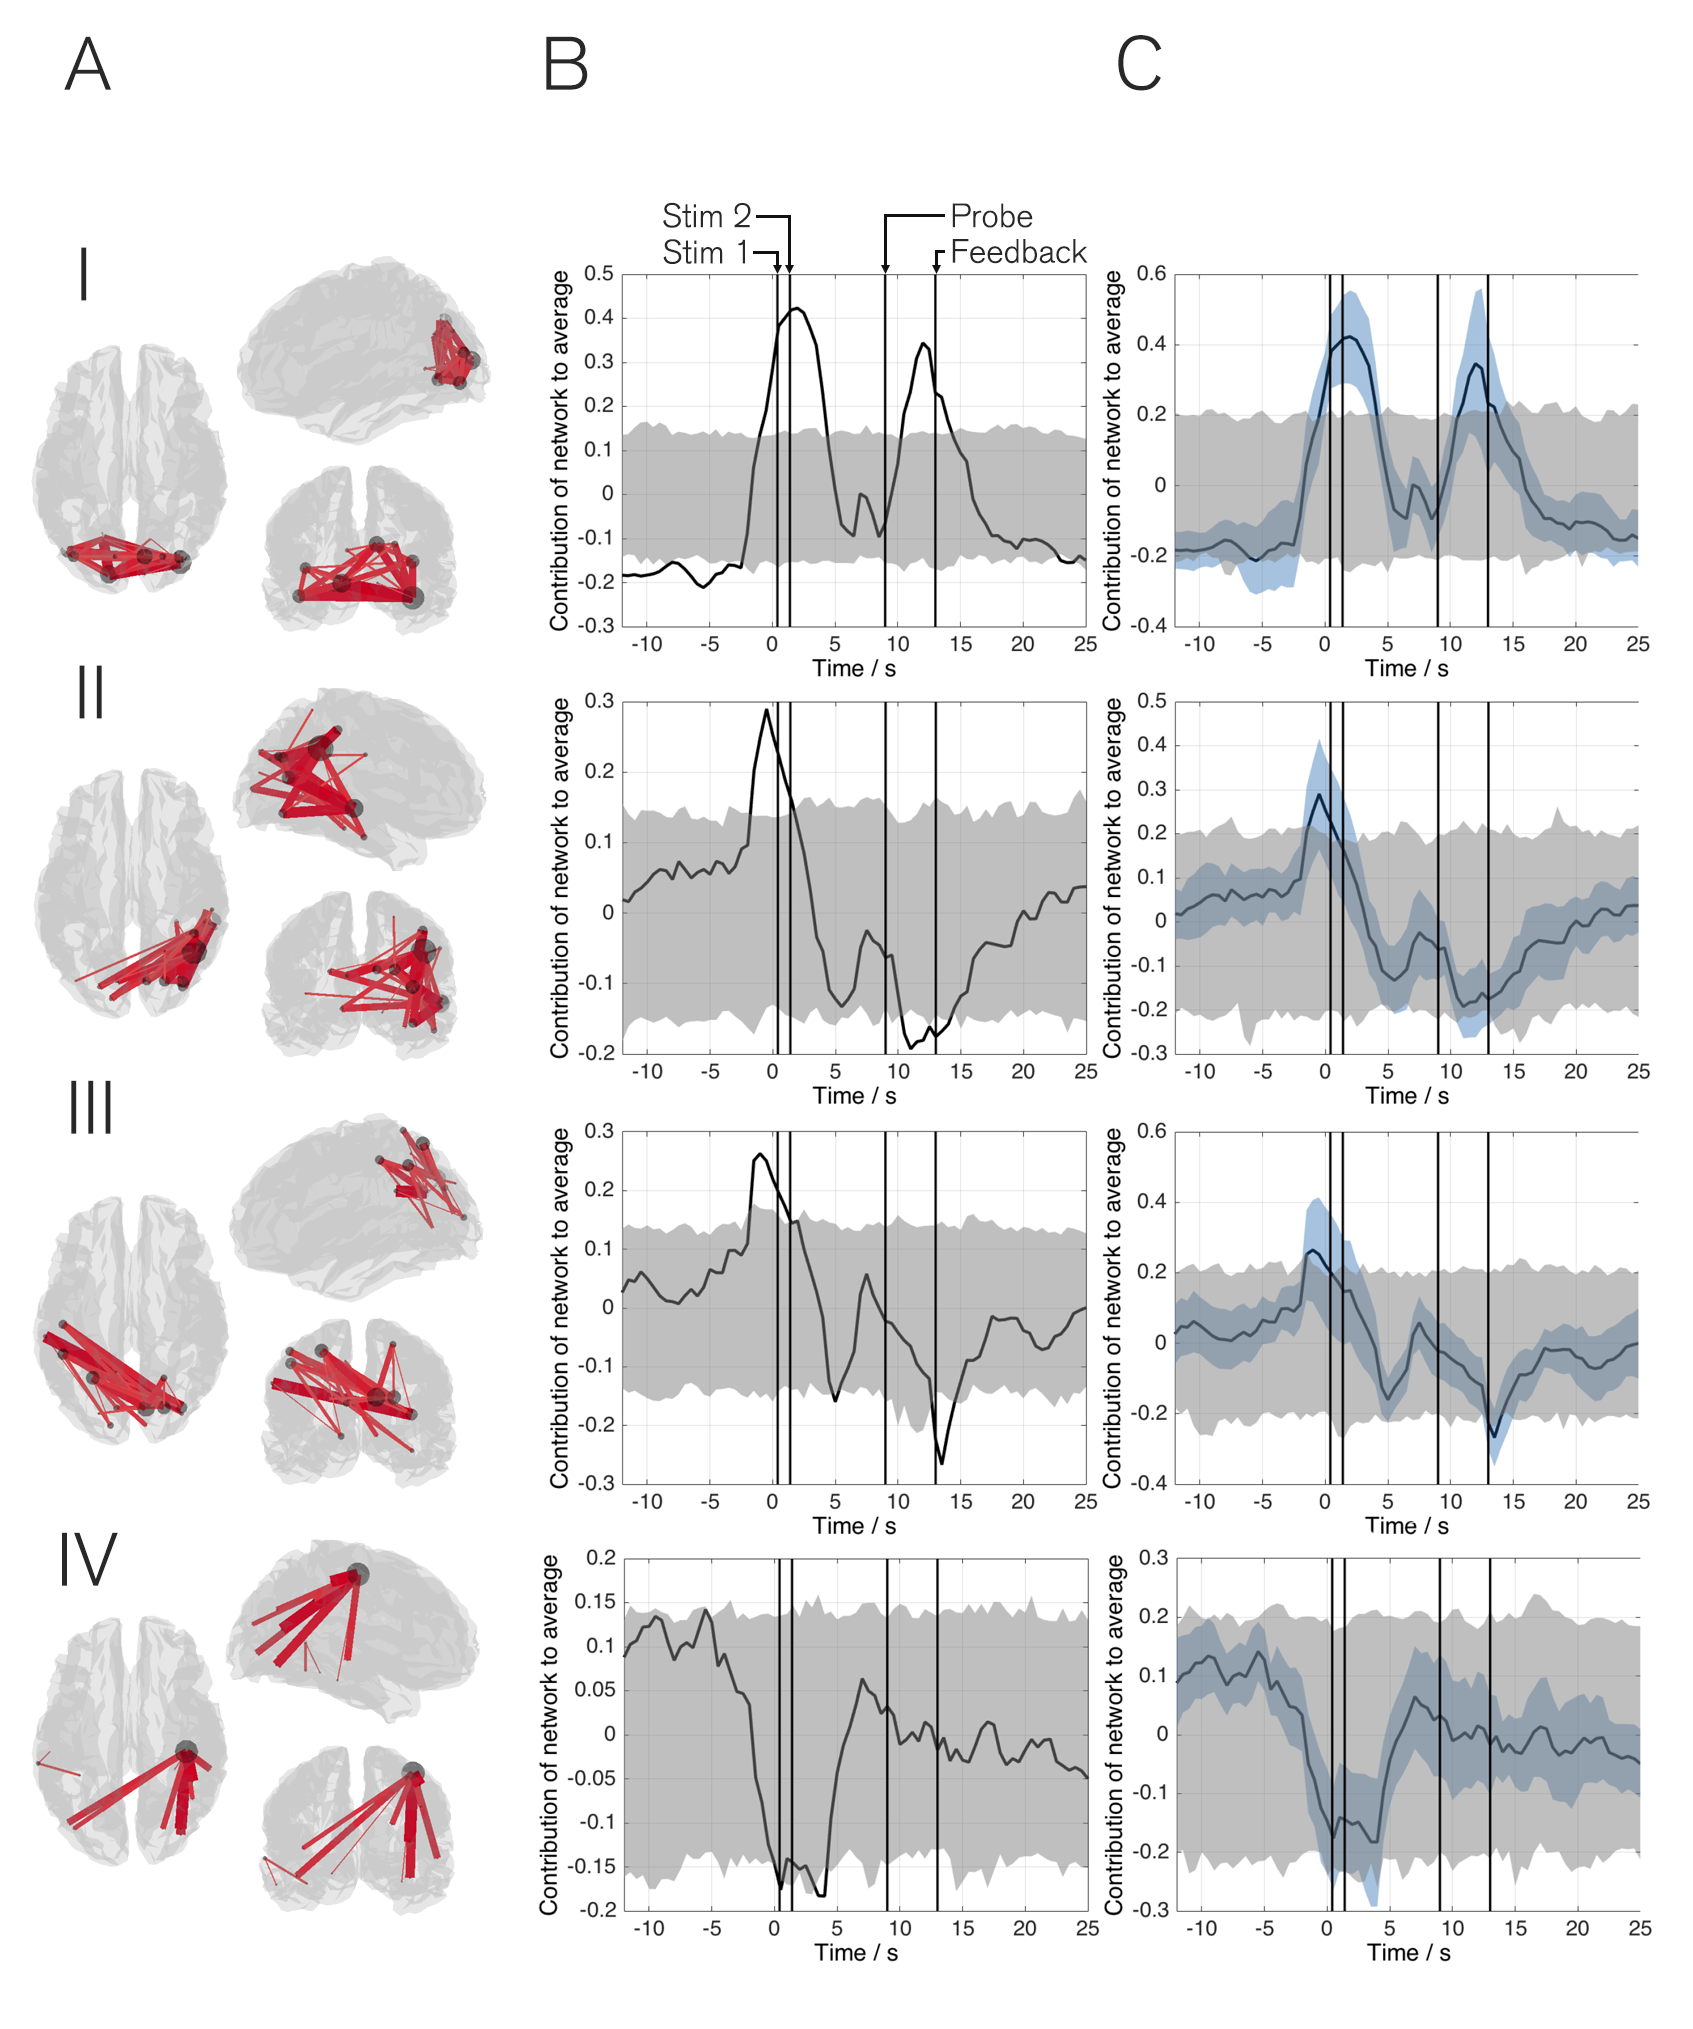
\includegraphics[width=\linewidth]{./images/chapter6/figure_3a.png}
			\caption{Results of the Sternberg experiment (part 1). The separate columns show A) 3D network visualisation. B) The average timecourse across 19 subjects. C) The split-half analysis. Rows I to IX show the 9 networks which modulate with the task, including I) primary visual; II) Visual to right tempero-parietal; III) Visual to left tempero-parietal; IV) Visuomotor. Note how the timings allow a temporal sequence of network involvement to be deduced.
		    \label{fig_6_3a}}
		\end{center}
	\end{figure*}
	
		\begin{figure*}[h!]
			\begin{center}
				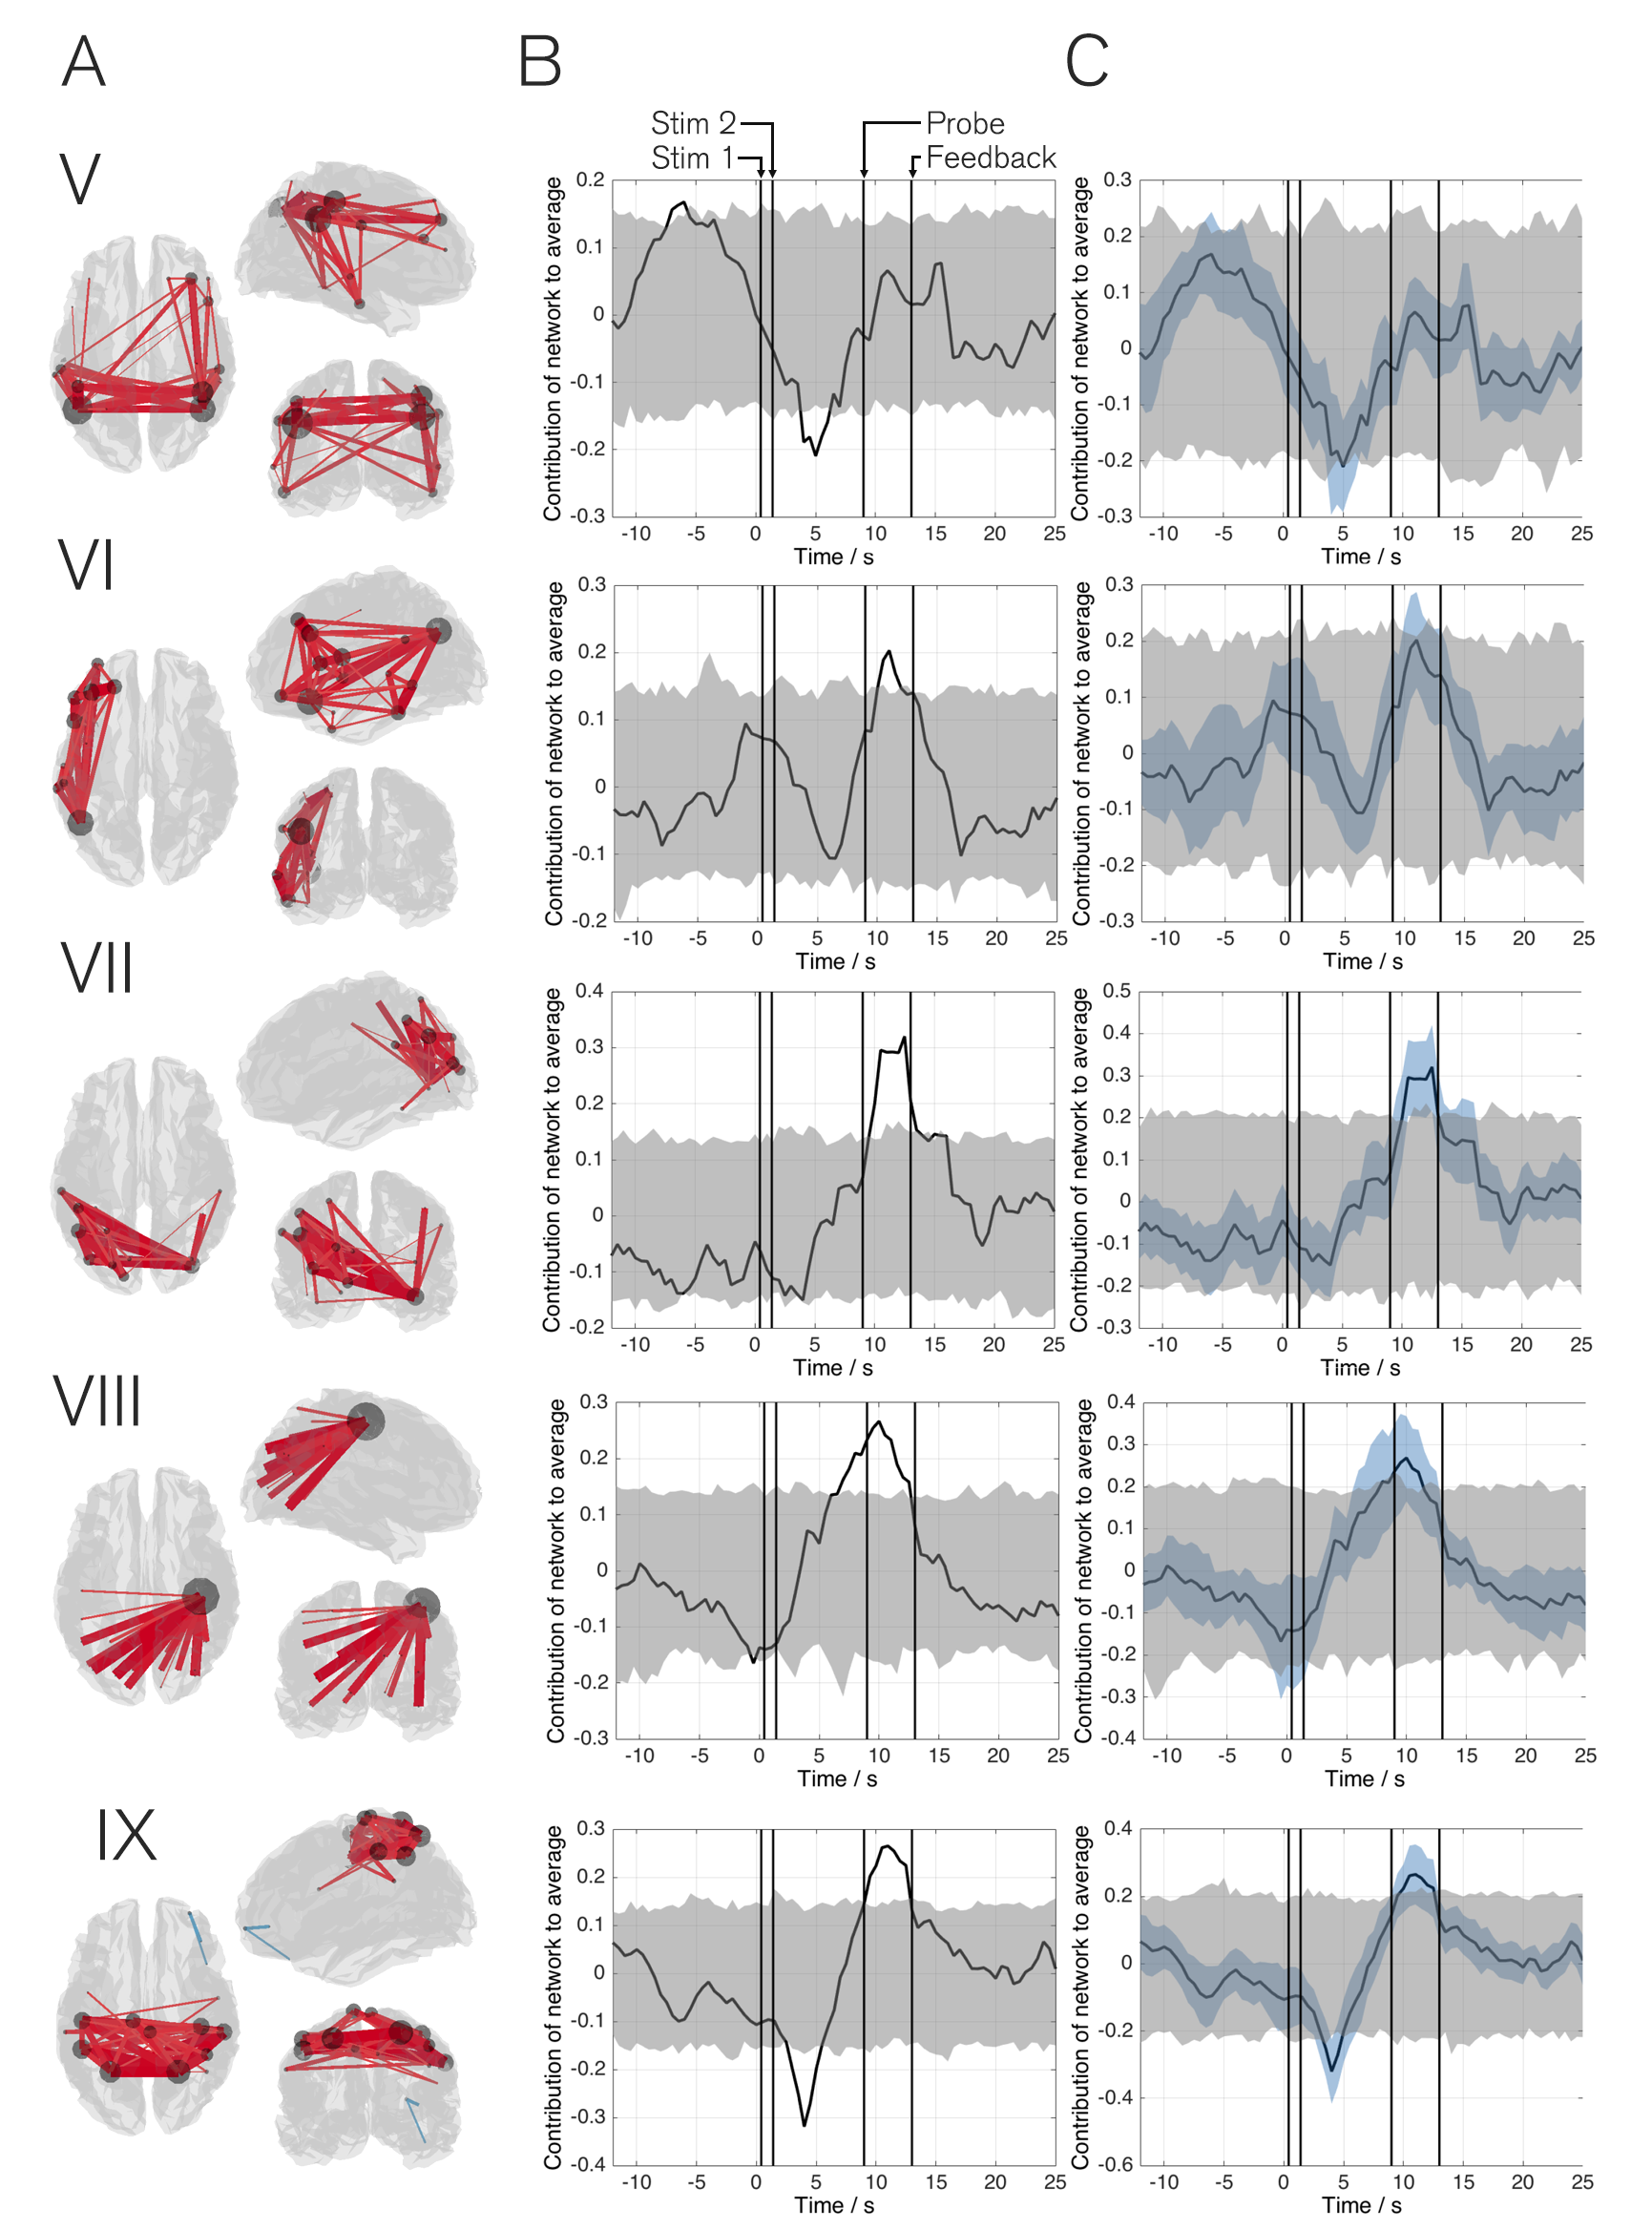
\includegraphics[width=\linewidth]{./images/chapter6/figure_3b.png}
				\caption{Results of the Sternberg experiment (part 2). The separate columns show A) 3D network visualisation. B) The average timecourse across 19 subjects. C) The split-half analysis. Rows I to IX show the 9 networks which modulate with the task, including V) Somantic; VI) Language; VII) Refined Visual to left tempero-parietal; VIII) Refined visuomotor; IX) Sensorimotor. Note how the timings allow a temporal sequence of network involvement to be deduced.
					\label{fig_6_3b}}
			\end{center}
		\end{figure*}

\section{Discussion}
This chapter has introduced a novel ICA based method which, when applied to MEG data, allows characterisation of transiently forming and dissolving electrophysiological networks in the brain, at time-scales much faster than could be achieved using fMRI. Previous MEG-ICA-network approaches typically look for brain regions whose activity, measured as a function of time, \textit{covaries}. Here distinct from this, we measure the temporal evolution of functional connectivity between regions and use temporal ICA to cluster together connections that share similar temporal profiles. In this way, we identify networks of connections whose temporal dynamics covary, with no prior assumptions regarding the brain regions involved. We have demonstrated our method using a simple finger movement task. Moreover, we have shown that our method allows generation of a unique picture of cognitive processing, showing clearly the formation and dissolution of multiple brain networks required to allow subjects to complete a Sternberg working memory task. 

The results generated by our method are of significant neuroscientific interest and warrant further discussion. However prior to this, two key points regarding the method should be understood: Firstly, the timecourses shown in Figures \ref{fig_6_2}, \ref{fig_6_3a} and \ref{fig_6_3b} depict increases and decreases in connectivity. In other words, the peaks refer to when two or more regions defining the network are most correlated. Just because regions are not connected at some particular point in time, does not necessarily mean that those regions are not actively engaged in the task. This is an important point since many of the regions implicated by our networks are likely to be engaged constantly throughout the Sternberg task, but may only connect to wider networks at specific points in time. Second, recall that there is inherent temporal smoothness in the method. Despite the excellent temporal resolution of MEG, a reasonable data window is required in order to derive reliably each individual adjacency matrix $\mathbf{R}_i$ (see also below). Here we employ a 6 s window width, meaning that a peak in a timecourse has an inherent uncertainty of ± 3 s. This means that, for example in the self-paced motor task where connectivity appears to increase before the button press, there is a degree of ambiguity; this could be representative of preparatory effects, or could result simply from the limited temporal resolution of the method. This temporal resolution is lower than other MEG based connectivity techniques, for example the Hidden Markov model introduced by \cite{Baker2014}. However this \pm 3 s resolution remains significantly higher than would be possible using techniques such as fMRI where a 6 s window would not facilitate sufficient data capture to accurately define connectivity. With these two considerations in mind it proves instructive to discuss the primary results of our method applied to the two datasets used. Figure \ref{fig_6_2} shows clearly that a network of brain connections involving primary motor cortices, as well as pre-motor and supplementary motor areas, can be identified based upon our self-paced finger movement task. Furthermore, this network of connections modulates significantly with the button press. Although simple, this result confirms the validity of our method by depicting clearly the primary motor and motor planning regions. The fact that no other networks modulate significantly with the task also helps to show that the method is capable of inferring networks that do not show task modulation. 

In the Sternberg task, the formation of networks encompassing visual (Figure \ref{fig_6_3a},I) and sensorimotor (IX) regions is consistent with the presentation of visual stimuli and execution of the motor response. Nodes in the occipital lobe typically include a lateral component which supports the notion that lateral occipital cortex (LOC) is specialised for object shape recognition \citep{Kourtzi2001}. Other networks encompass areas thought to be responsible for the higher level cognition required for successful completion of the Sternberg task. The Angular Gyrus (AG) is particularly evident in the majority of these networks. Structurally this region has been identified as a centrally connected hub serving multiple sub-networks. This hub has also been identified functionally in a variety of task-positive contexts ranging from semantic processing to numerical calculation.  A unified account of AG function is presented by \cite{Seghier2013} who suggests that the AG is an integration site receiving input from sensory, memorial and higher-level nodes. We speculate that the extent of our higher order networks is in agreement with this model of AG function. Notably, the dorso-lateral pre-frontal cortex (DLPFC) is recruited in network V, connecting bilaterally with the AG. The left and right DLPFC are well established in the literature as controlling executive-attention function in working memory \citep{Kane2002,Barbey2013}, with the right DLPFC being shown to be sensitive to shape in particular \citep{Nystrom2000}. This network also incorporates bilateral inferior temporal gyri, regions considered important for somantic processing \citep{Vigneau2006}. This leads us to name this network as a ‘semantic network’. A second cognitive network (VI) has been termed a ‘language network’. Although stimuli were abstract shapes, participant feedback suggests a ‘naming’ strategy was used in the majority of cases. If a verbalization strategy was employed by the participants to aid in memory encoding, then nodes of the language network may be implicated. Indeed, this left lateralised network is anchored in the AG with extensions to the inferior frontal gyrus (IFG), inferior temporal gyrus and a number of nodes spanning the inferior to superior precentral gyrus. These regions are consistent with previous accounts of somantic cognition \citep{Vigneau2006}. Furthermore, this effect was also seen by \cite{Caminiti2015} in their working memory task involving abstract shapes, and they also considered employment of a verbalisation strategy as a possible interpretation of the network activation. Finally, two networks (IV \& VIII) show ipsilateral motor connectivity with an extended network of occipital and parietal nodes. This is unusual considering the expected motor response would be in the contralateral hemisphere. However, the 4-30 Hz frequency band used encompassed alpha and beta oscillations and it is possible that, to suppress ipsilateral motor activity, alpha oscillations are increased \citep{Brinkman2014}. Overall, the transient networks induced by the Sternberg task are plausible given the previous literature on working memory and sensory processes.

\subsection{Methodological considerations}
Our algorithm allows detection and characterisation of transiently forming task induced electrophysiological networks. In achieving this, two core parameters require setting, the window width (here 6 s) and the number of independent components (here 10). Both warrant further discussion. A judicious selection of window width is important, and represents a trade-off between temporal resolution and the accuracy of the derived adjacency matrices. Here, separate elements of the adjacency matrices are based upon temporal correlation of envelope signals within the window. It is well known that the accuracy of correlation between two variables (\textit{r}) relates to the number of degrees of freedom ($η$) in the underlying data; specifically if one assumes no underlying genuine correlation between two timecourses then standard deviation of correlation, $σ(r)=1/\sqrt{η}$; i.e. the variability (noise) inherent in the adjacency matrices is increased as $η$ is decreased. Further, the number of degrees of freedom in a windowed envelope timecourse is unrelated to the number of sample points (or sampling frequency). In fact, Fourier theory shows that for envelope data, the upper limit on degrees of freedom is given by $N=B_w δ$, where $δ$ is the window width and $B_w$ represents bandwidth of the signal. This means that $σ(r)=1/\sqrt{B_w δ}$; in other words adjacency matrix noise is increased by either reducing bandwidth or window width. Typically bandwidth is set by the scientific question to be asked (e.g. one might be interested in beta band networks), and therefore $δ$ must be set to reduce the random noise to an acceptable level. Here $σ(r)=0.08$ which was deemed acceptable, however future studies should bear this calculation in mind when selecting window size. 

In addition to parameter selection, there are three other core components of the method that warrant discussion; namely, the choice of cortical parcellation, the underlying source space projection method, and the choice of connectivity metric. First, regarding the AAL parcellation, this was chosen based on its highly successful use in multiple previous MEG investigations (e.g. \citealp{Tewarie2016}). However, our method could be used with any cortical parcellation provided that the number of regions is sufficiently low, and those regions are sufficiently well separated, to ensure that the windowed data matrices, $\mathbf{Q}_i$, are of full rank. It is noteworthy that the separate AAL regions vary markedly in size, meaning that our use of a single point location, based on the centre of mass of the region, may mean that some regions are better represented than others. The future use of brain parcellations based directly on MEG data may therefore prove instructive. For example, we could generate a functional atlas based on the functional hubs highlighted in applications of CCA in multiple resting state networks or apply CCA between AAL parcels to break them down into functionally specific ROIs.   

Secondly, we chose an envelope correlation procedure as our estimator of functional connectivity between regions. This procedure has been successful in elucidating electrophysiological networks of functional connectivity \citep{Colclough2016}, particularly in the study of the electrophysiological basis of haemodynamic networks \citep{Tewarie2016}. However, other methods (for example those based on fixed phase measurements between regions) are available; these should not be considered competitor techniques but rather they probe a different type of functional connectivity \citep{Scholvinck2013}. For example, using a time-varying multivariate autoregressive model, it has been demonstrated that task-dependent brain states can be identified in a finger tapping task, and correspond to unique cross-spectral (i.e. coherence) patterns \citep{Vidaurre2016}. Although at present this method this is limited (computationally) to pairs of brain areas, whereas our method in this chapter is whole-brain. The two methods may be combined in the future. Indeed, the adjacency matrices derived in our methodology could easily be substituted for similar adjacency matrices derived using any alternative metric (assuming sufficiently high signal to noise ratio), and transient networks probed.

Finally, we note that there is significant variability in our results across subjects. The cross-subject variability was shown by our split half analysis and was a consistent finding throughout the chapter, occurring in the Sternberg as well as the self-paced experiment. In fact, relatively poor within and between subject reliability of (static) MEG connectivity measurements has been shown previously. For example, \cite{Wens2014a} show that whilst group level static connectivity within several well-known distributed networks is stable, there is significant variability at the individual subject level. Similarly \cite{Colclough2016} tested the cross session repeatability of a large number of static functional connectivity measurements, showing clearly that although group level inference is reliable, network metrics can be very variable across individuals. In addition, \cite{Tewarie2016} used MEG networks to predict those observed in fMRI; whilst predictions were robust at the group level, they fared less well within individuals. Interestingly, these variations across subjects may not be due to stochastic noise, but rather identifiable intrinsic processes which are subject specific \citep{Finn2015}.  Given these previous findings of large inter-individual differences in static connectivity, it is not surprising that dynamic functional connectivity metrics presented here also exhibit relatively high inter-individual differences. There are a number of possible explanations for this. Firstly, our measurement of connectivity itself (i.e. the dynamic adjacency matrices) are based only on 6 s of unaveraged MEG data.  Given the relatively low SNR of MEG data it is possible that reliability is only realised with large quantities of data – hence the requirement for large subject cohorts. Second, source localisation could affect the robustness of connectivity; here we use beamforming alongside the AAL atlas, a technique well established by previously published work. However, a limitation is that if a specific region, e.g. left motor cortex, is mislocalised (e.g. due to a poor forward model in one subject) then the signal derived would no longer be representative of that region. This potential confound would add markedly to variability over subjects. Thirdly, the reliability of the amplitude envelope correlation metric itself could be questioned. However, \cite{Colclough2016} showed that of all of the MEG based connectivity metrics, AEC fared well in terms of robustness over repeated measures. Finally, this variability could genuinely reflect the variability across individual subjects in terms of the neural network mechanisms used to carry out the tasks undertaken. Ultimately, if techniques like the one presented here are to be useful clinically, then we must derive means to ensure their robustness in individuals. Further effort is thus need in this area.


\section{Conclusions}

In the context of this thesis, this investigation may at first glance appear to stand separate to Chapters \ref{chapter_cca} and \ref{chap_kmeans}, as its approach to functional connectivity analysis is markedly different. However the results support the same hypothesis about dynamic electrophysiological brain networks, these networks will rapidly form and dissolve to support ongoing cognitive function, even at larger spatial scales. Previous MEG-ICA network analyses look for brain regions that share a common temporal profile of activity. Here distinctly, we measure the temporal evolution of connectivity between region pairs and use ICA to identify clusters of connections that share an independent temporal profile. The validity of our method was demonstrated in a self-paced finger movement paradigm, showing that a motor network can be distinguished. The broader applicability of our method was demonstrated by its application to a Sternberg task. We have shown that our method allows generation of a unique picture of cognitive processing, showing clearly the formation and dissolution of the brain networks required to allow subjects to complete the task. This represents a significant step forward in the characterisation of brain network connectivity and will prove to be a key tool in the future investigation of healthy brain networks, and their breakdown in a variety of pathological conditions.
\clearpage

\appsection
\section{APPENDIX A: Additional Self Paced Results}\label{sec_atlas_appendix_A}
\begin{figure}[h!]
	\includegraphics[width=\linewidth]{./images/chapter6/s1a.png}\caption{Networks from self paced motor analysis not shown in main manuscript (1-5). The separate columns show A) 3D network visualisation. B) The average timecourse across 10 subjects. C) The split-half analysis. Note that rows I and II show significant modulation of connectivity across all subjects but fail to in the split half analysis.}
\end{figure}
\begin{figure}[h!]
	\includegraphics[width=\linewidth]{./images/chapter6/s1b.png}\caption{Networks from self paced motor analysis not shown in main manuscript (6-9). The separate columns show A) 3D network visualisation. B) The average timecourse across 10 subjects. C) The split-half analysis.}
\end{figure}
